\chapter{Anexo}
\label{cap:Anexo}

\begin{figure}[h!]
  \centering
  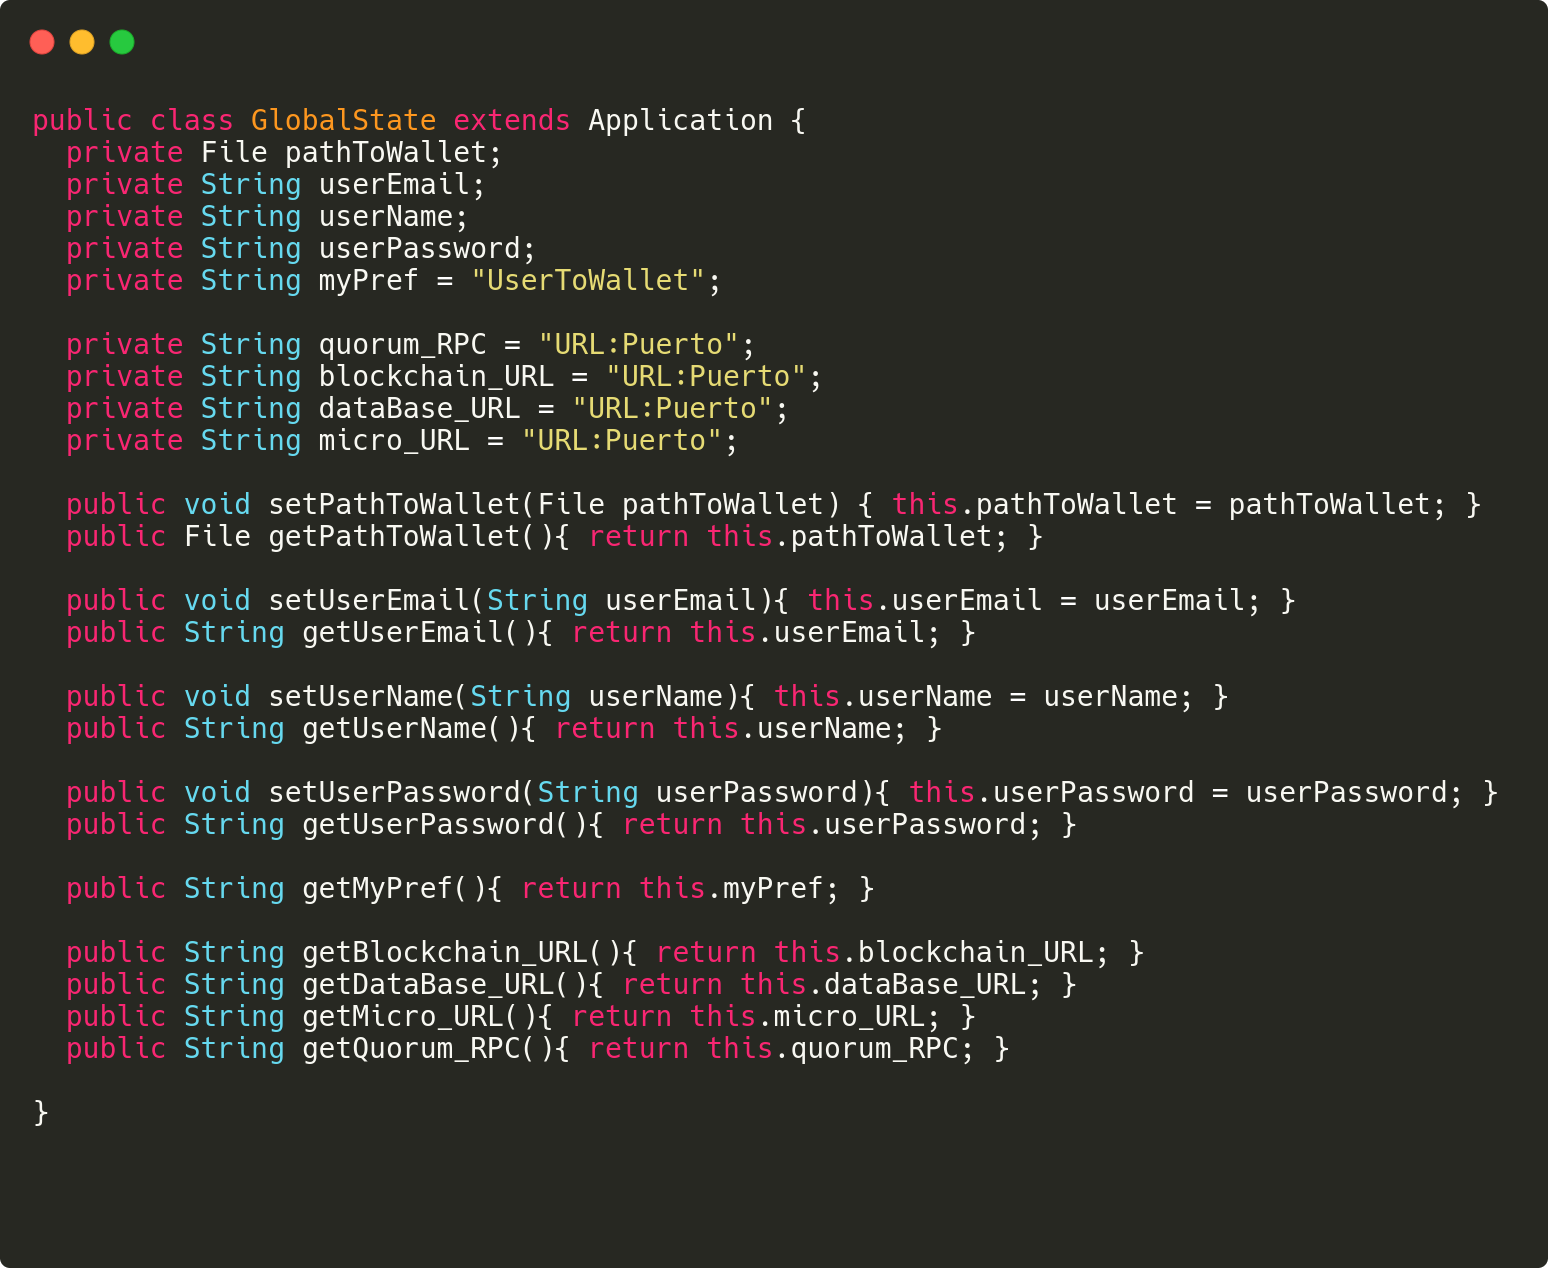
\includegraphics[width=1\linewidth]{figs/Anexo/gs}
  \caption[Código de GlobalState]{Código de GlobalState}
  \label{fig:gs}
\end{figure}

\begin{figure}[h!]
  \centering
  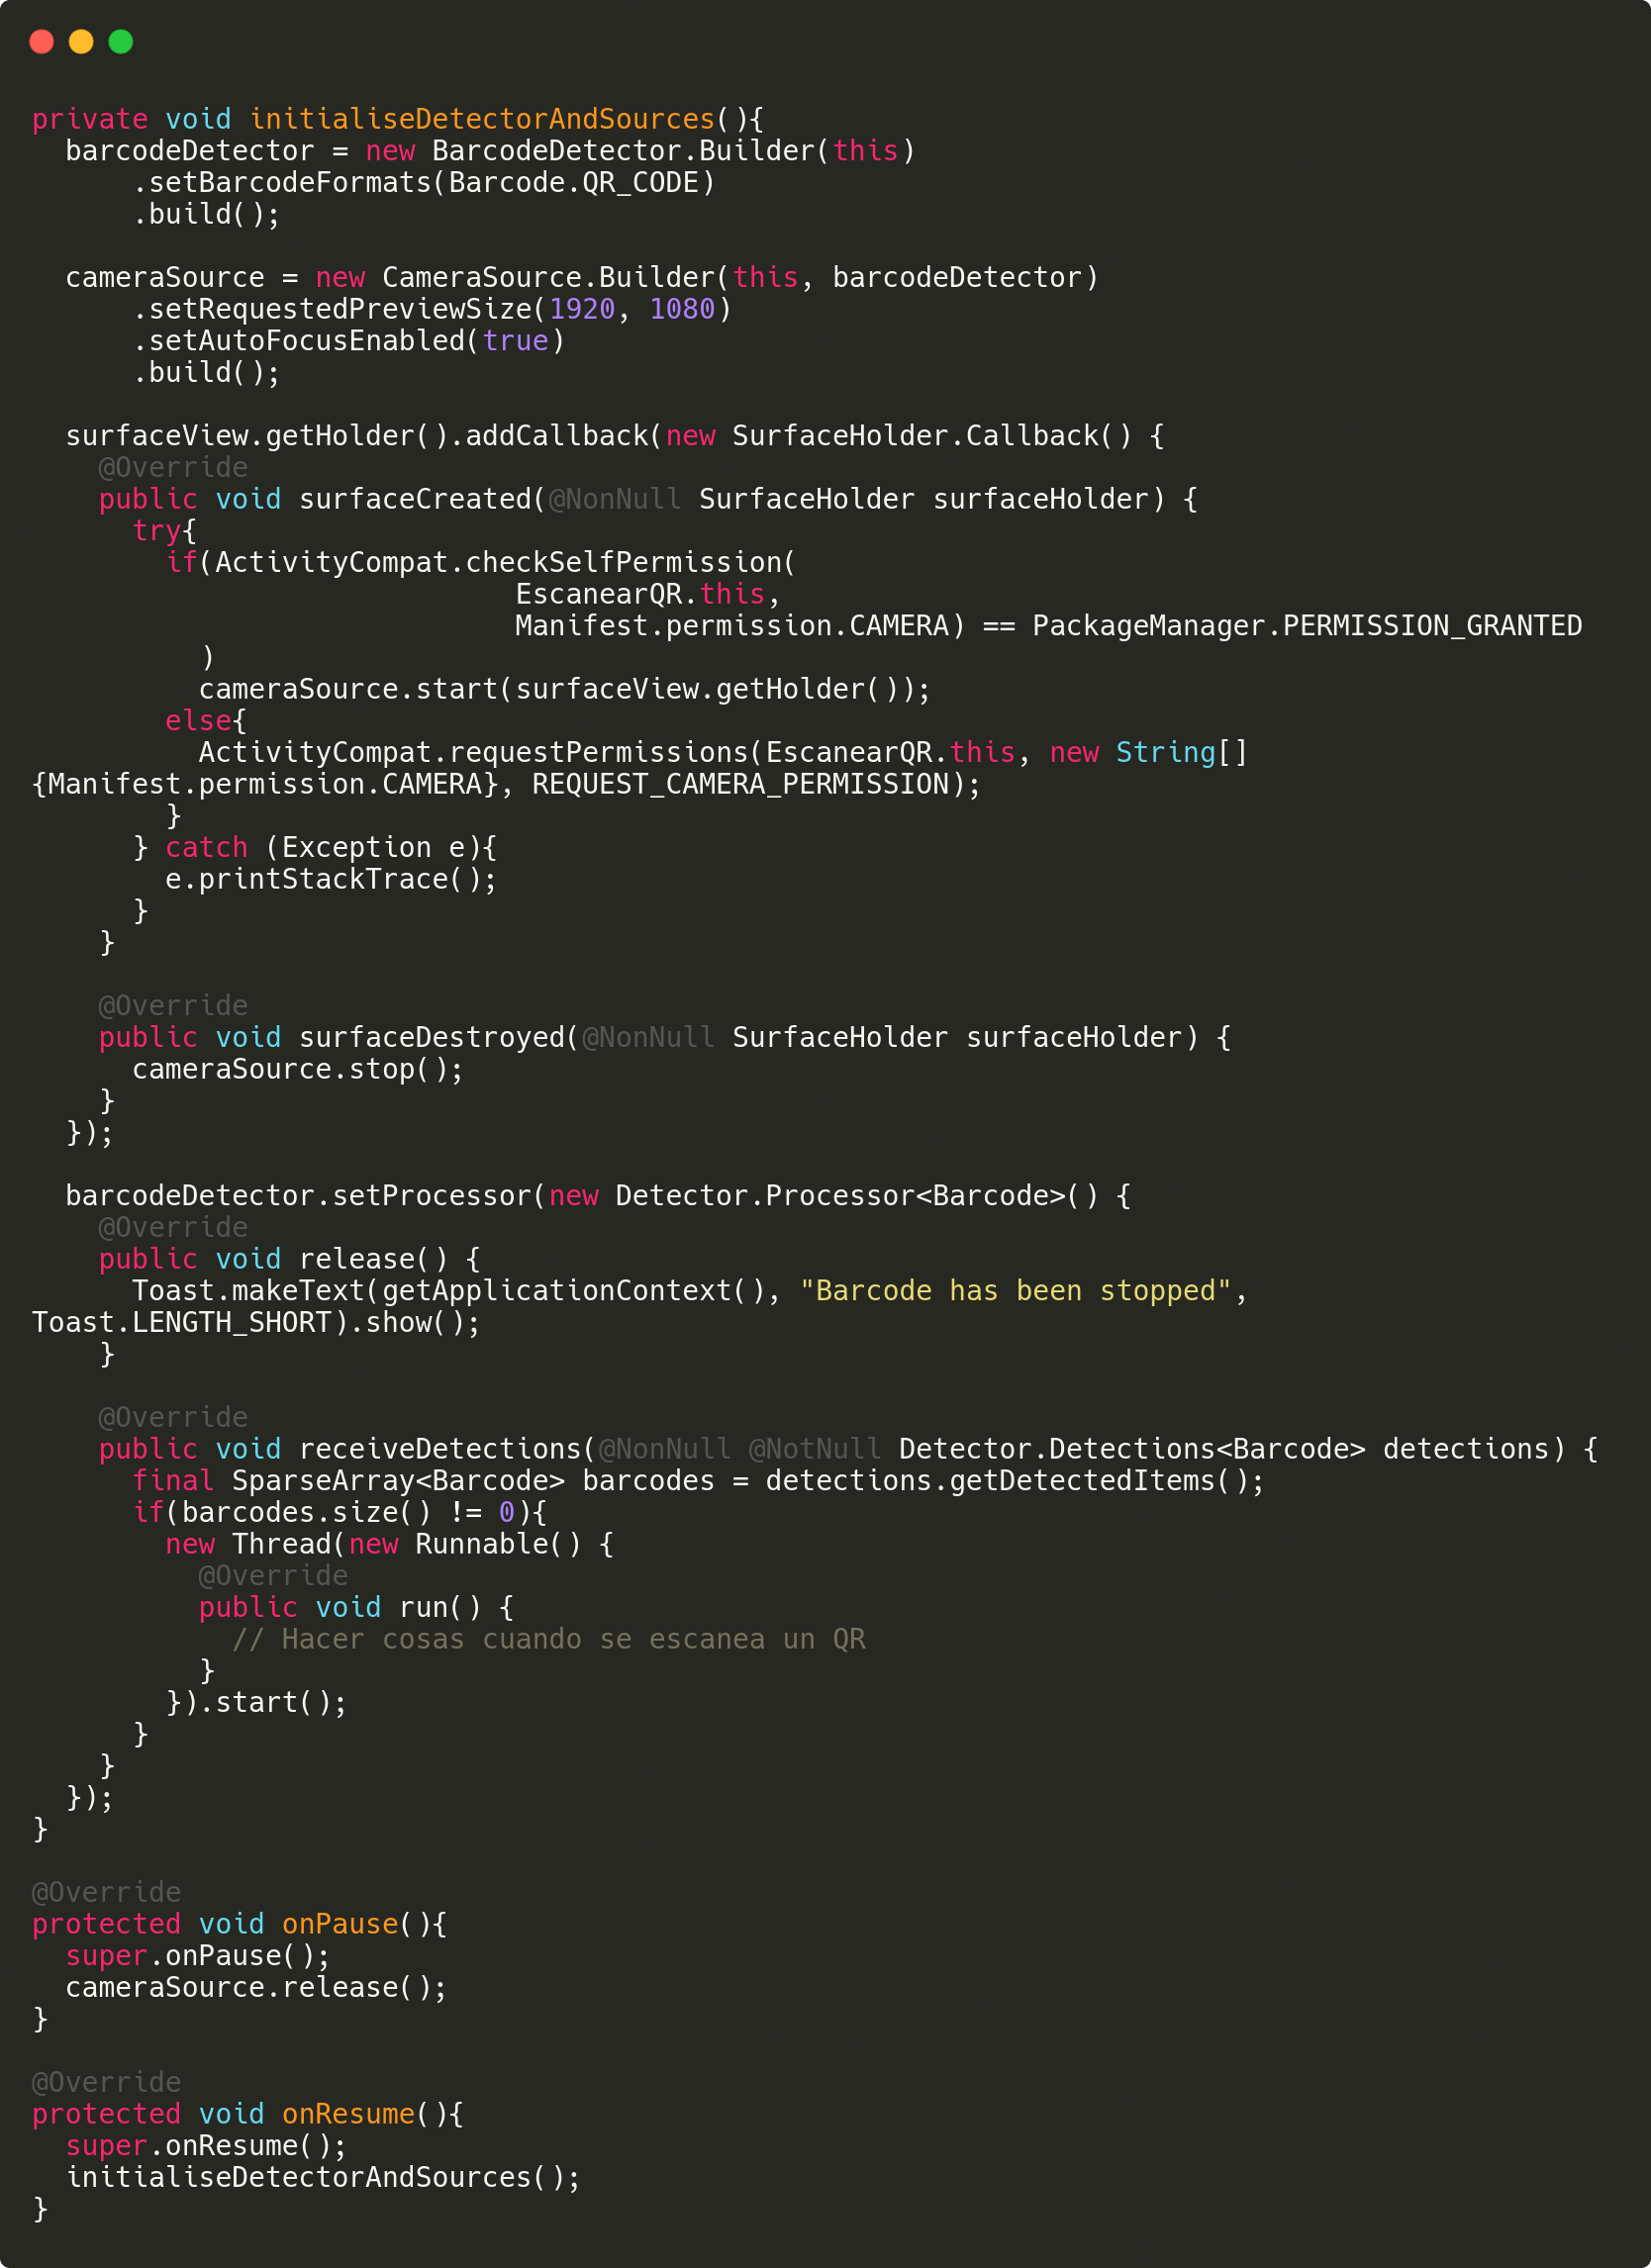
\includegraphics[width=1\linewidth]{figs/Anexo/zxing}
  \caption[Código del escaneado de QRs]{Código del escaneado de QRs}
  \label{fig:escaneandoQRs}
\end{figure}

\begin{figure}[h!]
  \centering
  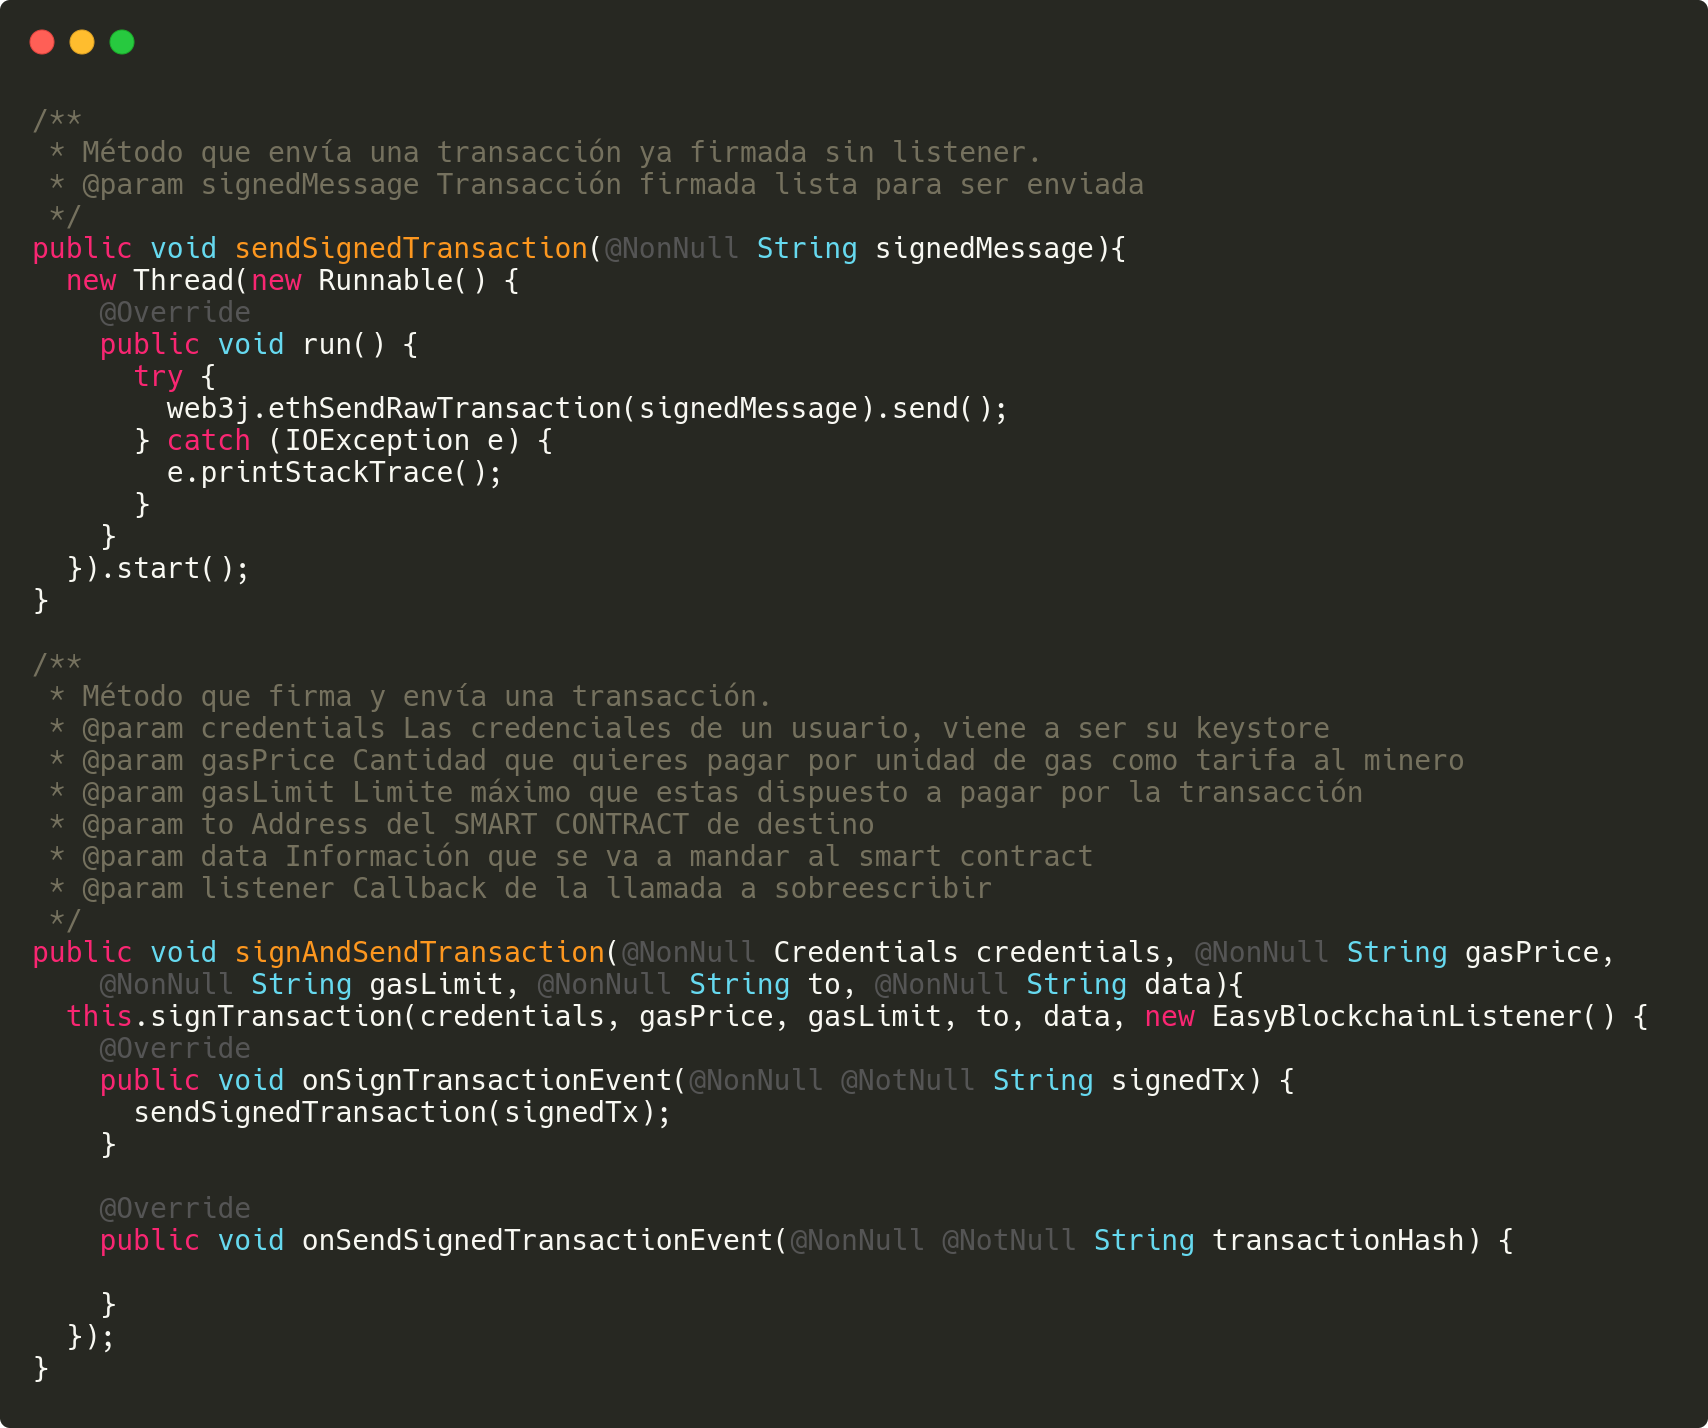
\includegraphics[width=1\linewidth]{figs/Anexo/firma_envia_completo}
  \caption[Firmado y enviado de una transacción]{Firmado y enviado de una transacción}
  \label{fig:firma_envia_completo}
\end{figure}

\begin{figure}[h!]
  \centering
  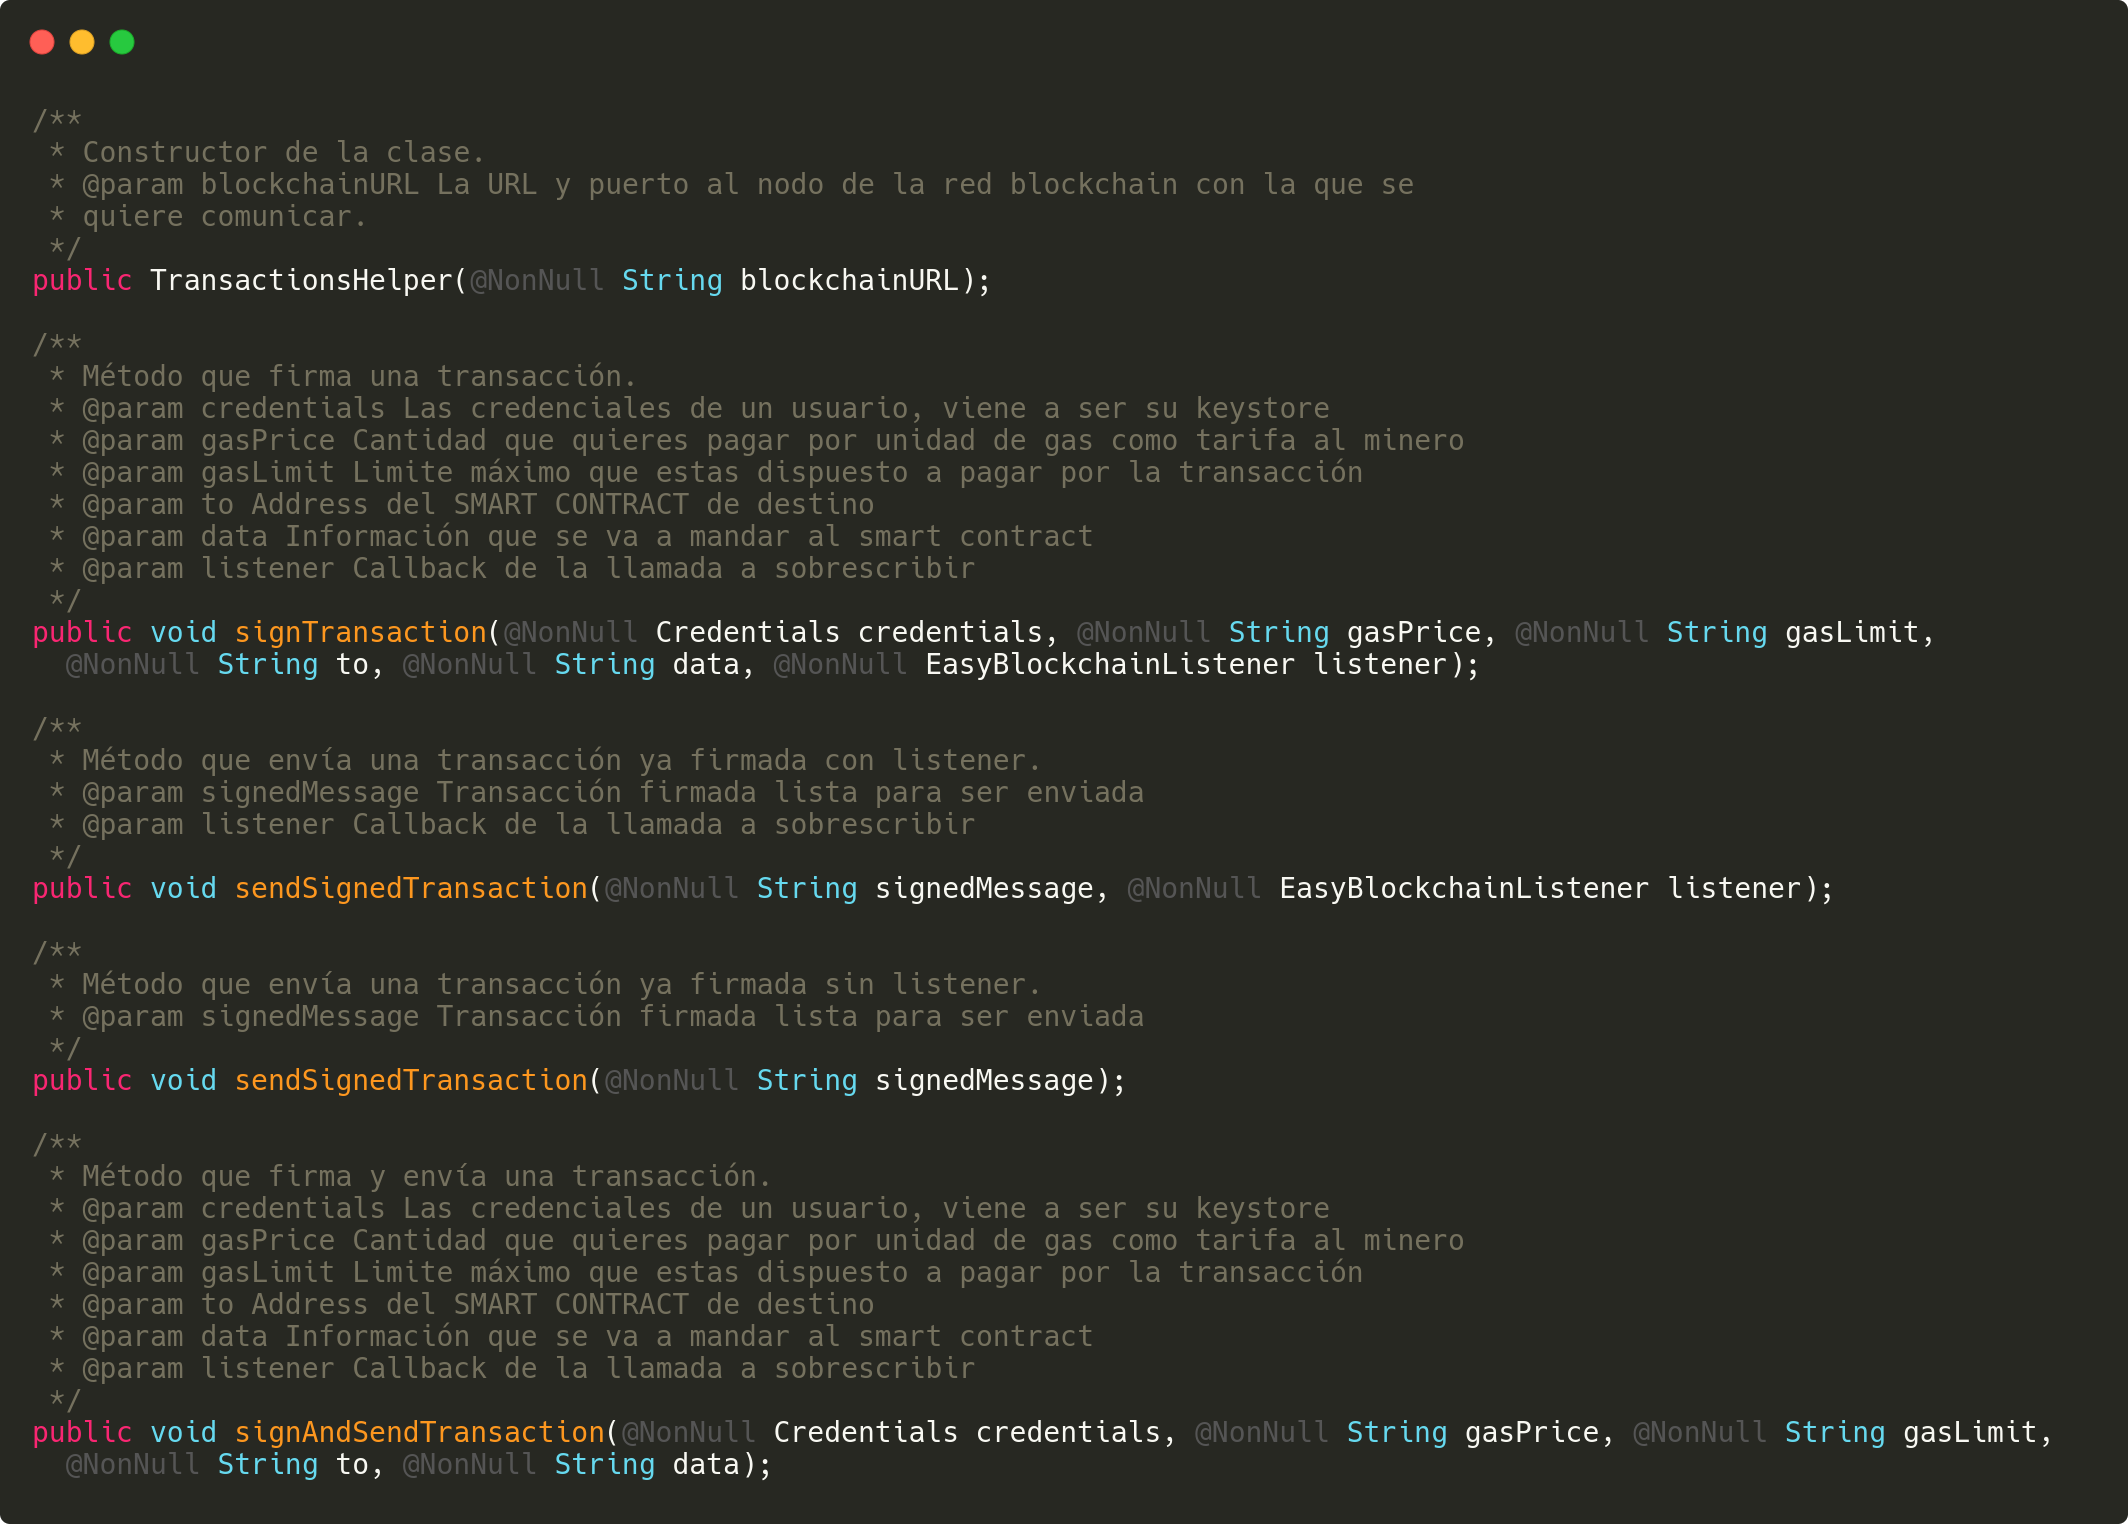
\includegraphics[width=1\linewidth]{figs/Anexo/Docs/trans}
  \caption[Documentación de TransactionsHelper]{Documentación del TransactionsHelper}
  \label{fig:docsTransHelper}
\end{figure}

\begin{figure}[h!]
  \centering
  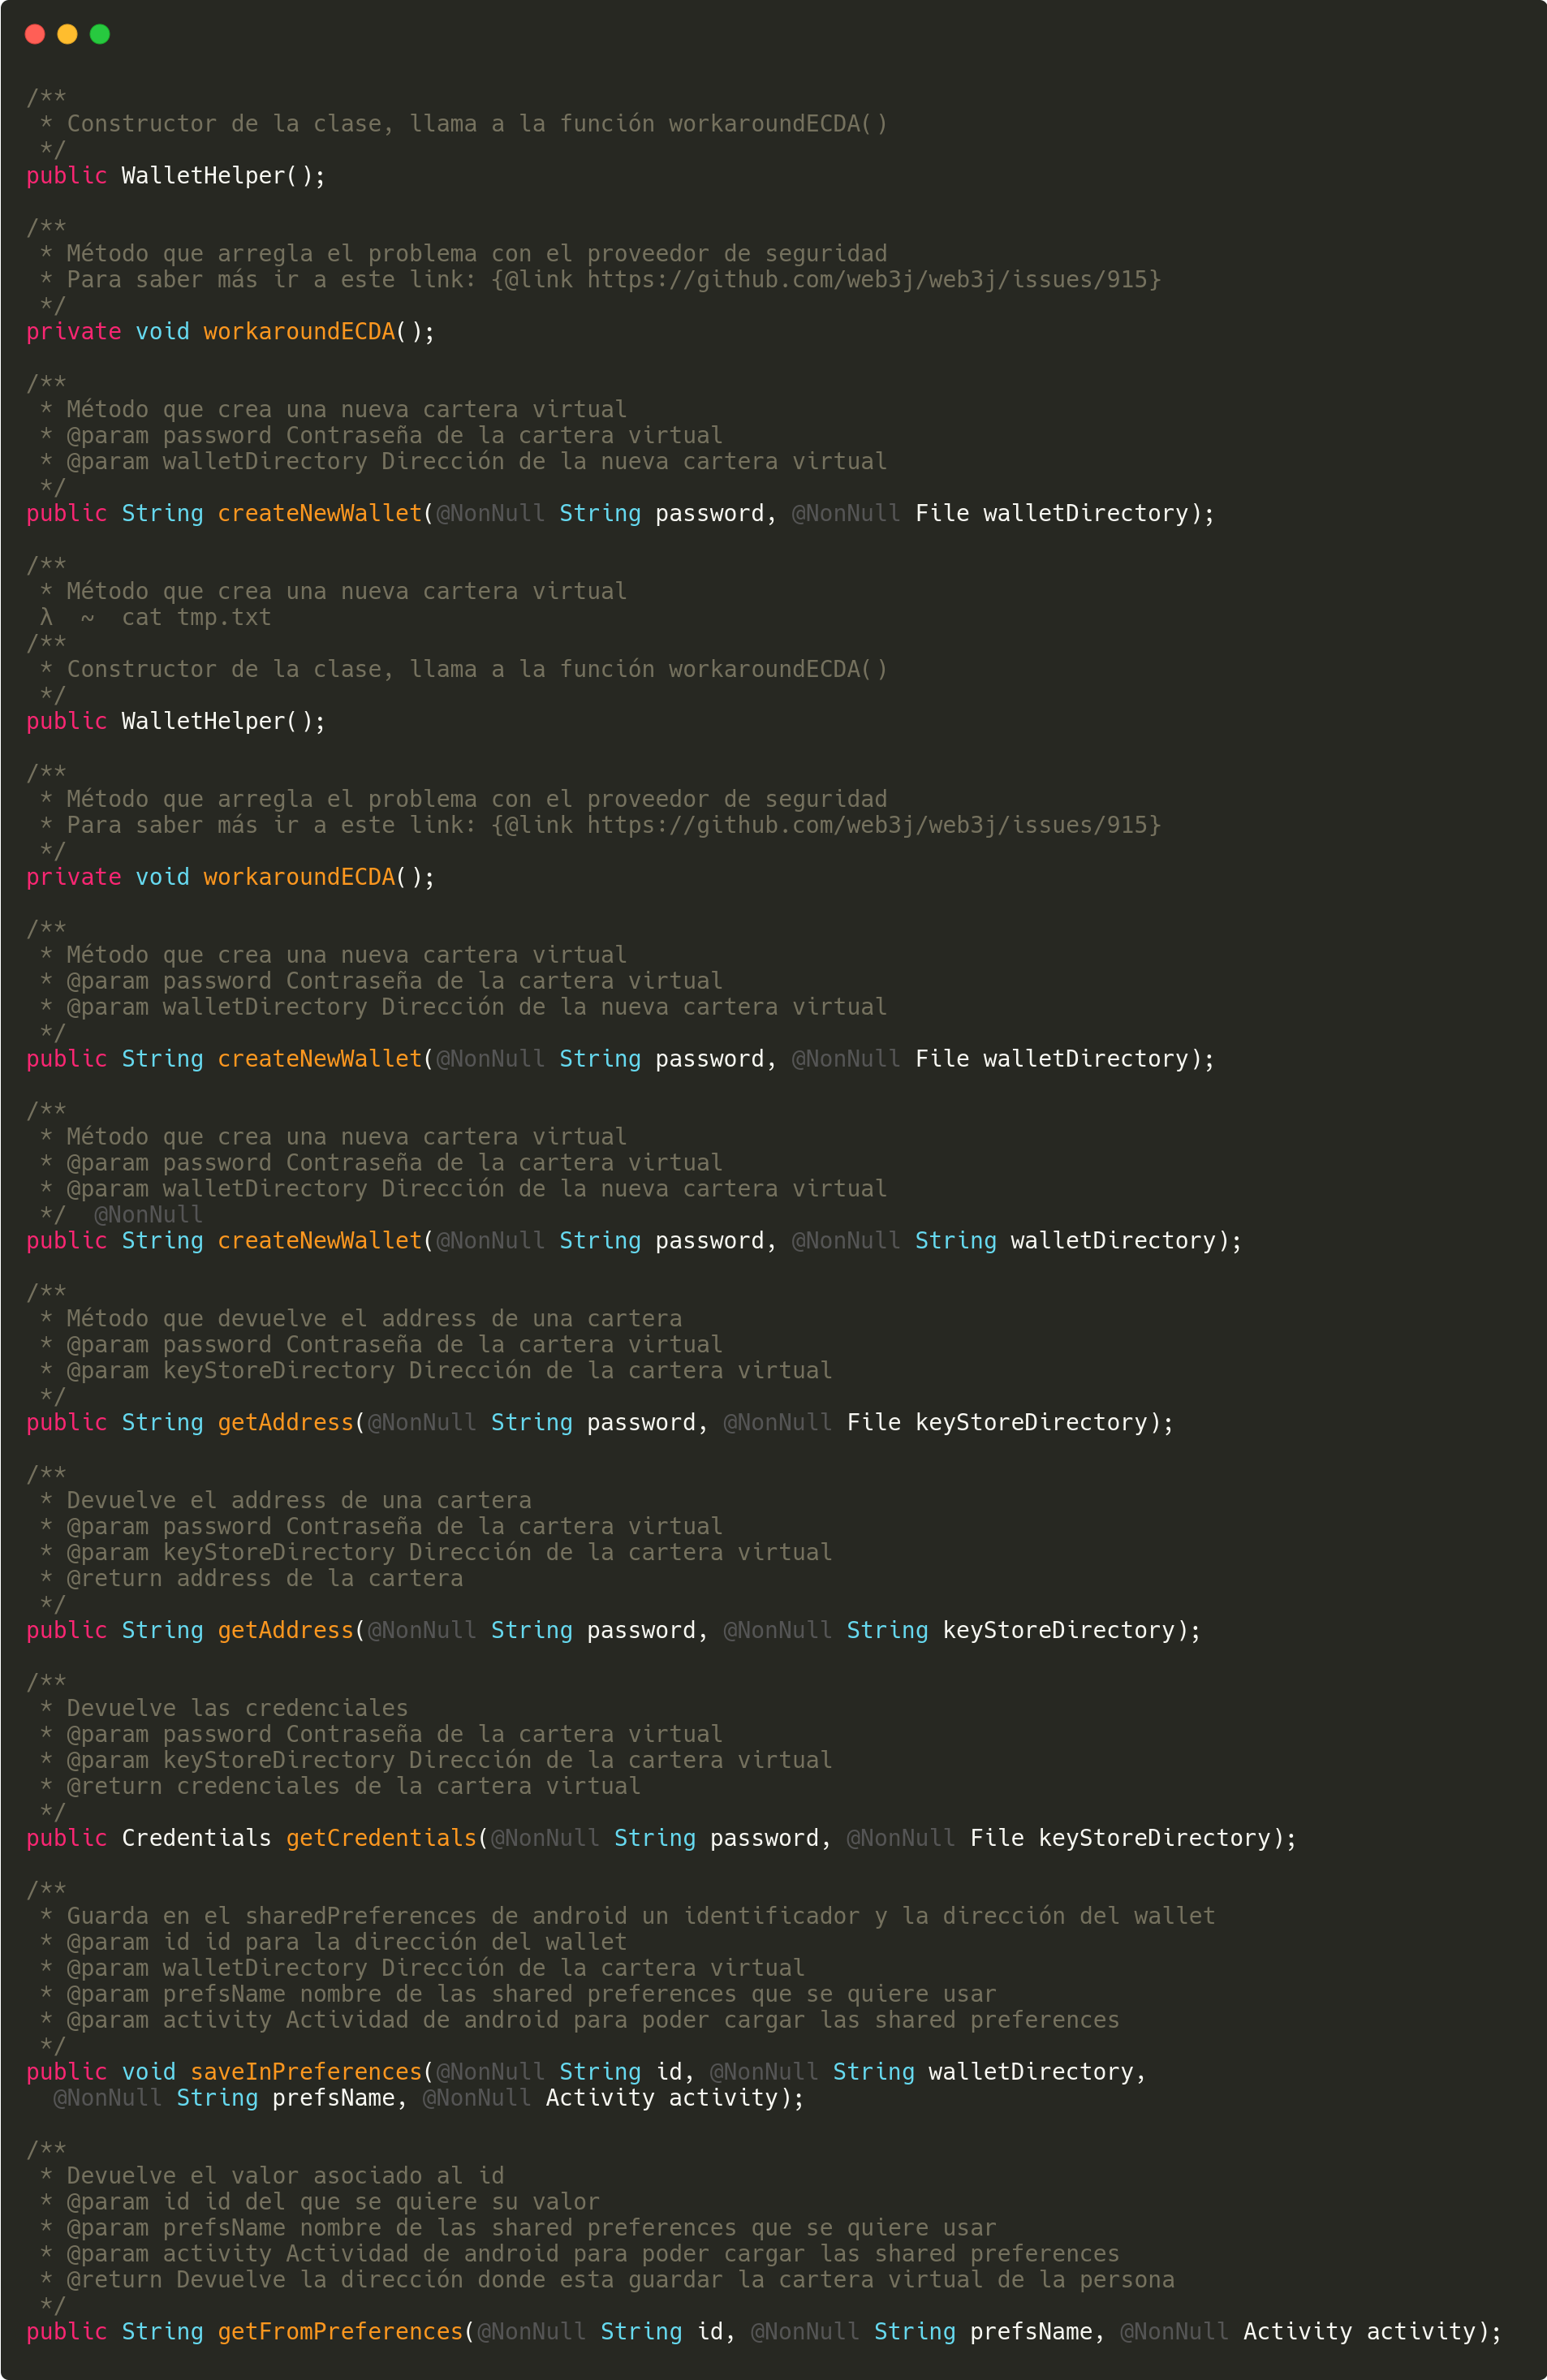
\includegraphics[width=1\linewidth]{figs/Anexo/Docs/wallet}
  \caption[Documentación de WalletHelper]{Documentación del WalletHelper}
  \label{fig:docsWalletHelper}
\end{figure}

\begin{landscape}
\begin{figure}[h!]
  \centering
  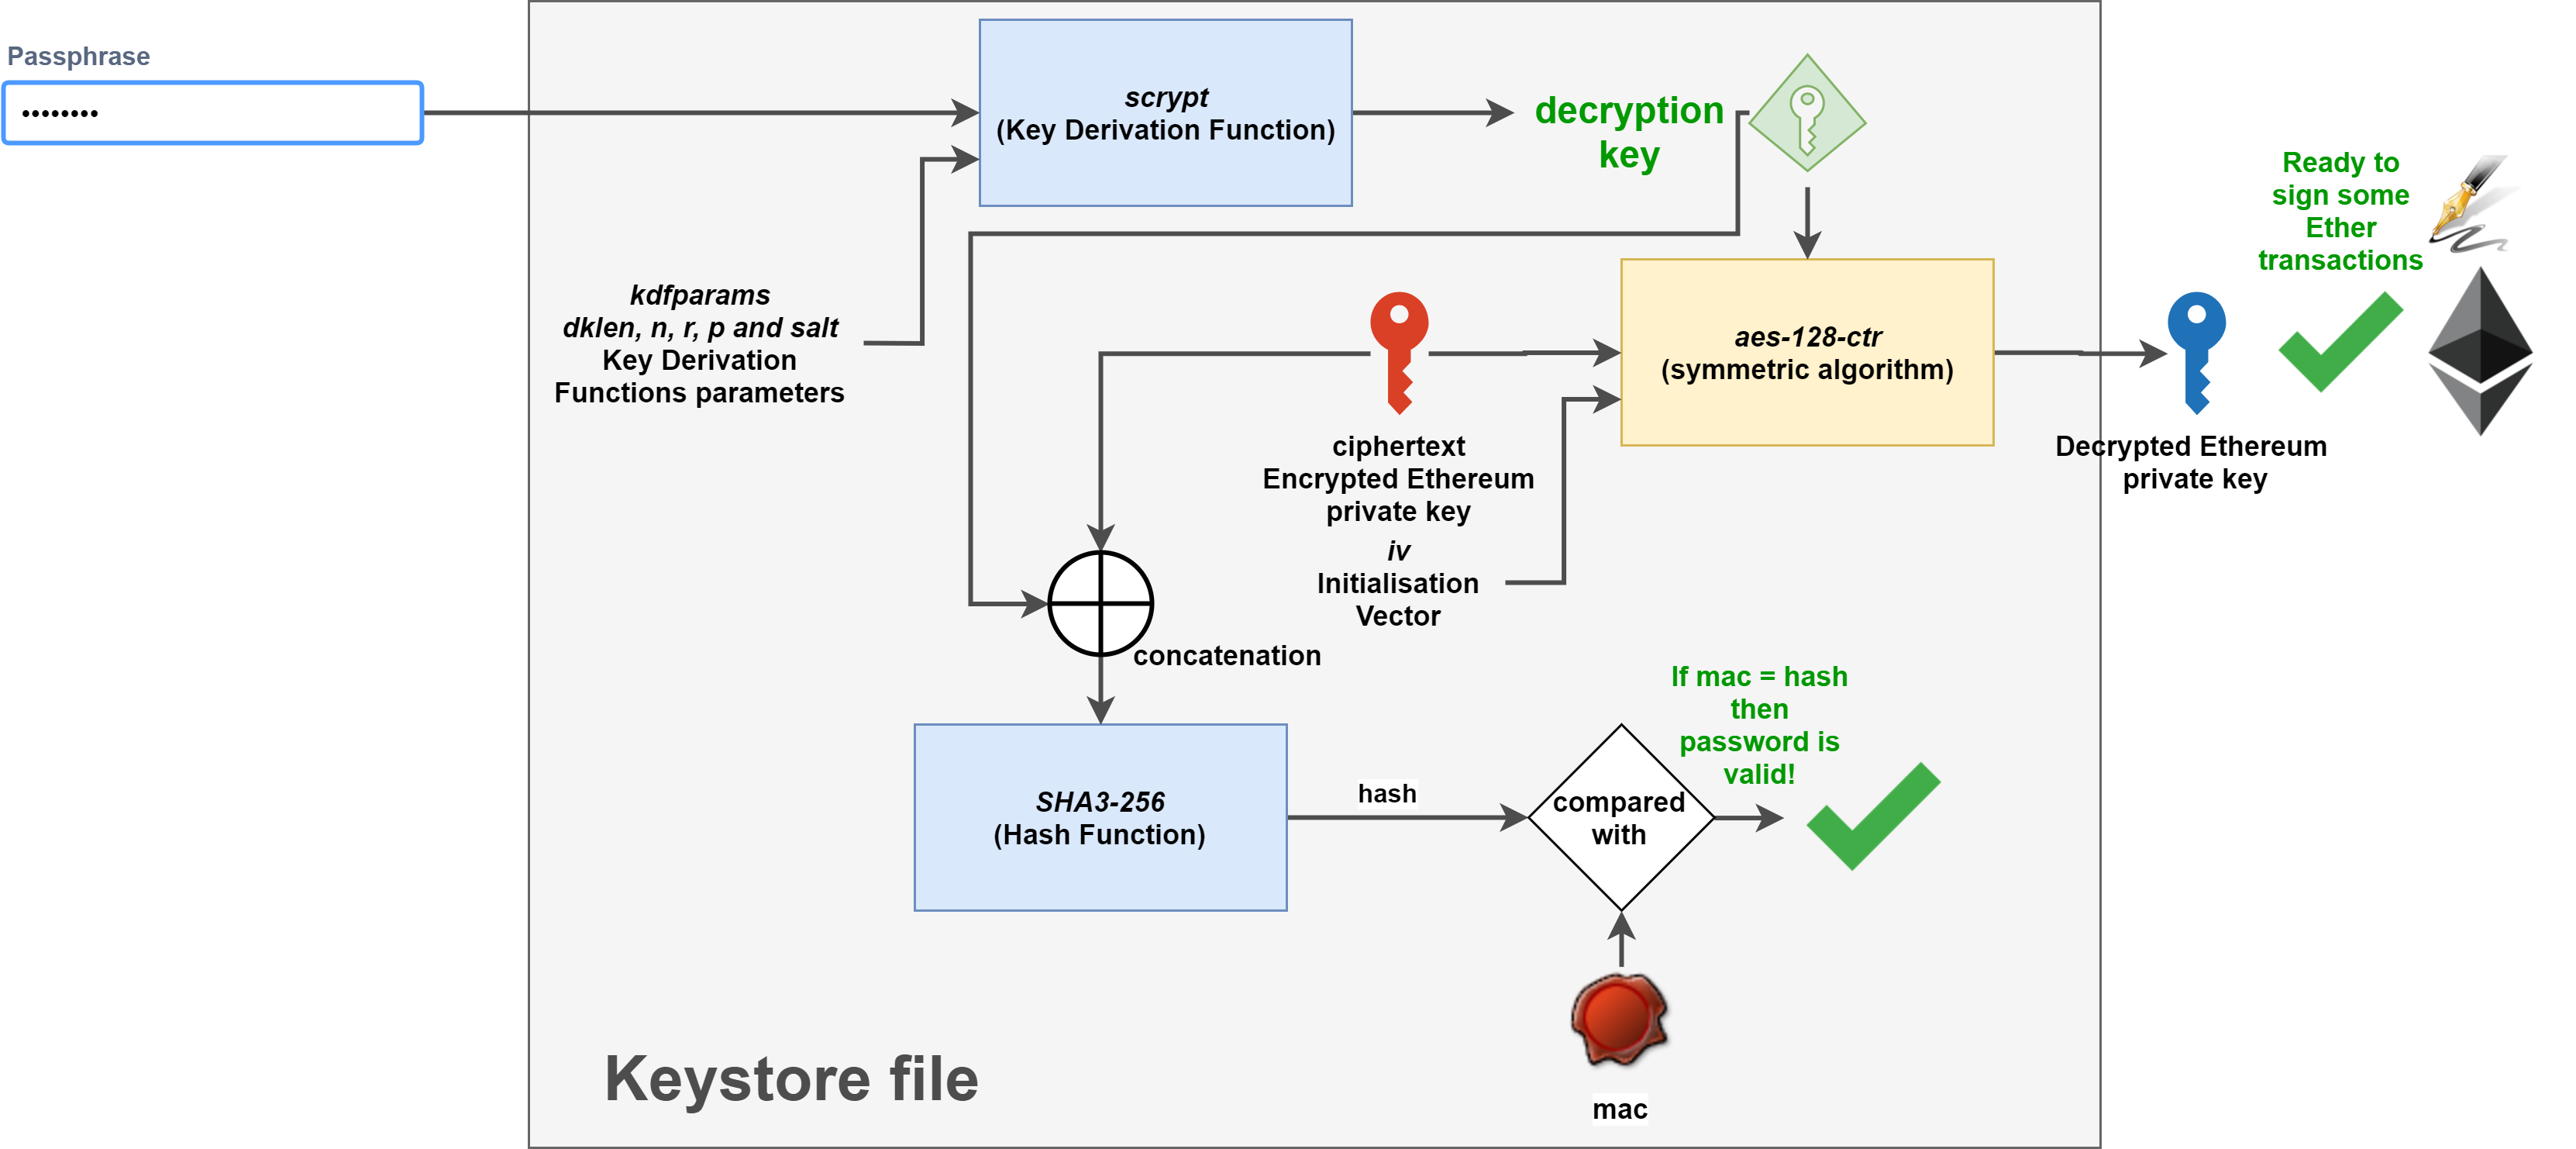
\includegraphics[scale=0.2]{figs/Anexo/keystore_completo}
  \caption[Flujo completo del funcionamiento de un keystore]{Flujo completo del funcionamiento de un keystore (\href{https://julien-maffre.medium.com/what-is-an-ethereum-keystore-file-86c8c5917b97}{Julian M})}
  \label{fig:keystore_completo}
\end{figure}
\end{landscape}
